\documentclass[12pt]{article}
\usepackage{geometry}                % See geometry.pdf to learn the layout options. There are lots.
\geometry{letterpaper}                   % ... or a4paper or a5paper or ... 
%\geometry{landscape}                % Activate for for rotated page geometry
%\usepackage[parfill]{parskip}    % Activate to begin paragraphs with an empty line rather than an indent
\usepackage{float}
\usepackage{graphicx}
\graphicspath{{images/}}
\usepackage{amsmath,amssymb,amsfonts,amsthm} 
\usepackage{epstopdf}
\usepackage{cleveref}
\usepackage{epigraph}

% Computer Concrete
%\usepackage{concmath}
%\usepackage[T1]{fontenc}

% Times variants
%
\usepackage{mathptmx}
\usepackage[T1]{fontenc}
%
%\usepackage[T1]{fontenc}
%\usepackage{stix}
%
% Needs to typeset using LuaLaTeX:
%\usepackage{unicode-math}
%\setmainfont{XITS}
%\setmathfont{XITS Math}

% garamond
%\usepackage[cmintegrals,cmbraces]{newtxmath}
%\usepackage{ebgaramond-maths}
%\usepackage[T1]{fontenc}

\DeclareGraphicsRule{.tif}{png}{.png}{`convert #1 `dirname #1`/`basename #1 .tif`.png}

\theoremstyle{plain}
\newtheorem{theorem}{Theorem}
\newtheorem{corollary}[theorem]{Corollary}
\newtheorem{lemma}[theorem]{Lemma}
\newtheorem{proposition}[theorem]{Proposition}
\newtheorem{conjecture}[theorem]{Conjecture}
\newtheorem{question}[theorem]{Question}

\theoremstyle{definition}
\newtheorem{definition}[theorem]{Definition}
\newtheorem{example}[theorem]{Example}
\newtheorem*{keywords}{Keywords}
\newtheorem*{sources}{Sources}
\newtheorem*{todo}{TODO}

\theoremstyle{remark}
\newtheorem{remark}[theorem]{Remark}
\newtheorem{note}[theorem]{Note}

\title{Autocorrelation}
\author{Nhan Trong}
\date{\today}                                           % Activate to display a given date or no date

\begin{document}
\maketitle

\epigraph{\textit{If you want to find the secrets of the universe, think in terms of energy, frequency and vibration.}}{Nikola Tesla}

\begin{keywords}
Standard, cuberoot and enhanced autocorrelation.
\end{keywords}

\begin{question}
Can you use autocorrelation to detect speech events?
\end{question}

It appears you can. E.g. Audacity has an implementation called Standard Autocorrelation, which we can apply to non-vocal and vocal segments of an audio:

\begin{figure}[H]
\centering
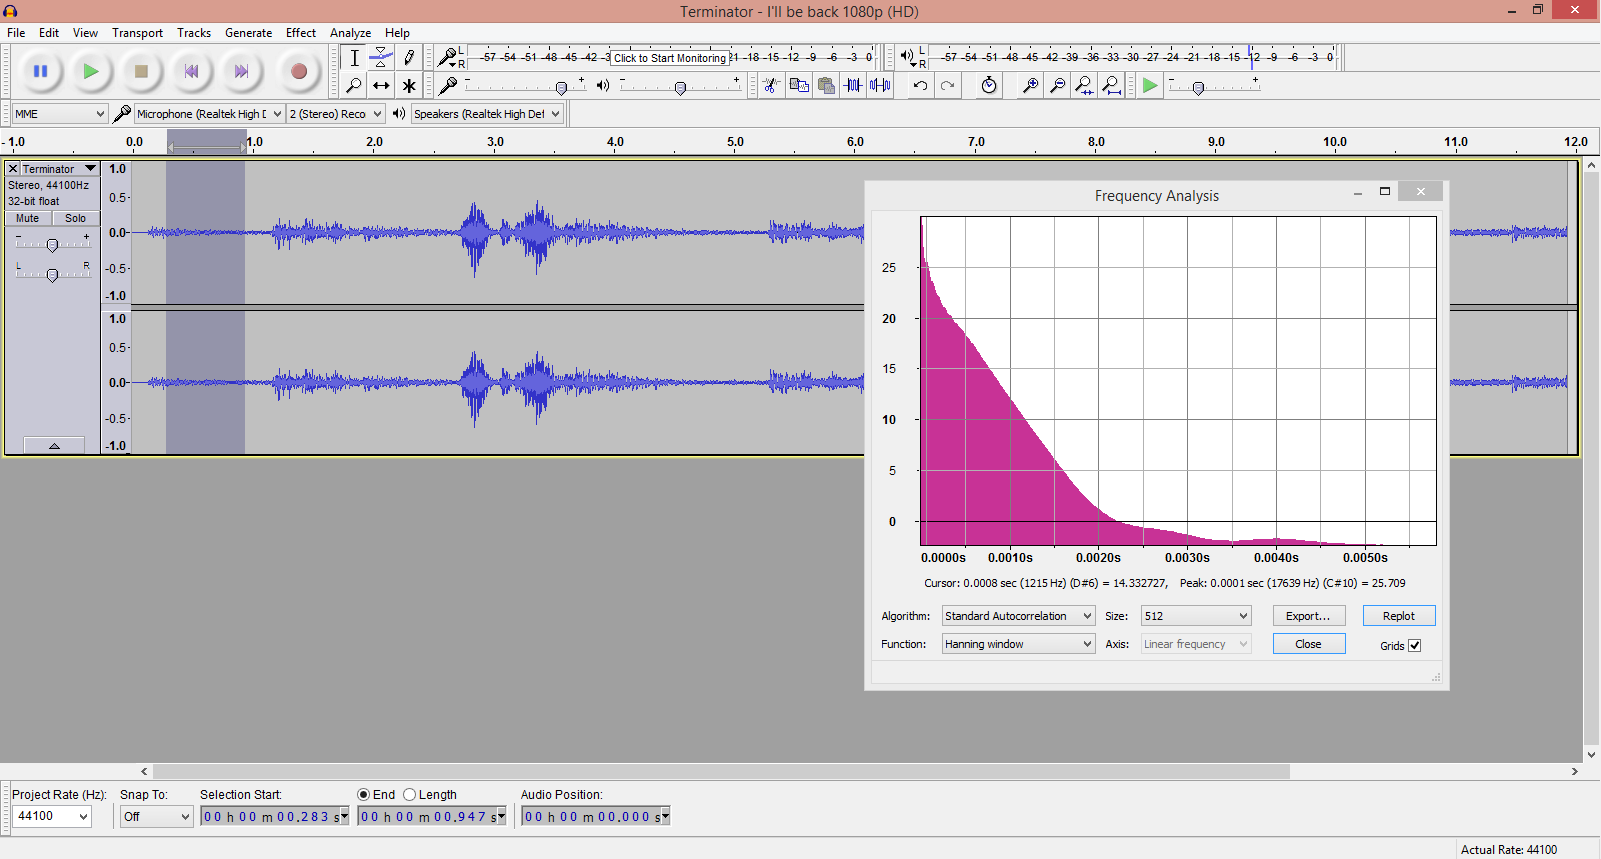
\includegraphics[width=1.0\textwidth]{autocorrelation1}
\caption{Non-vocal autocorrelation}
\end{figure}

\begin{figure}[H]
\centering
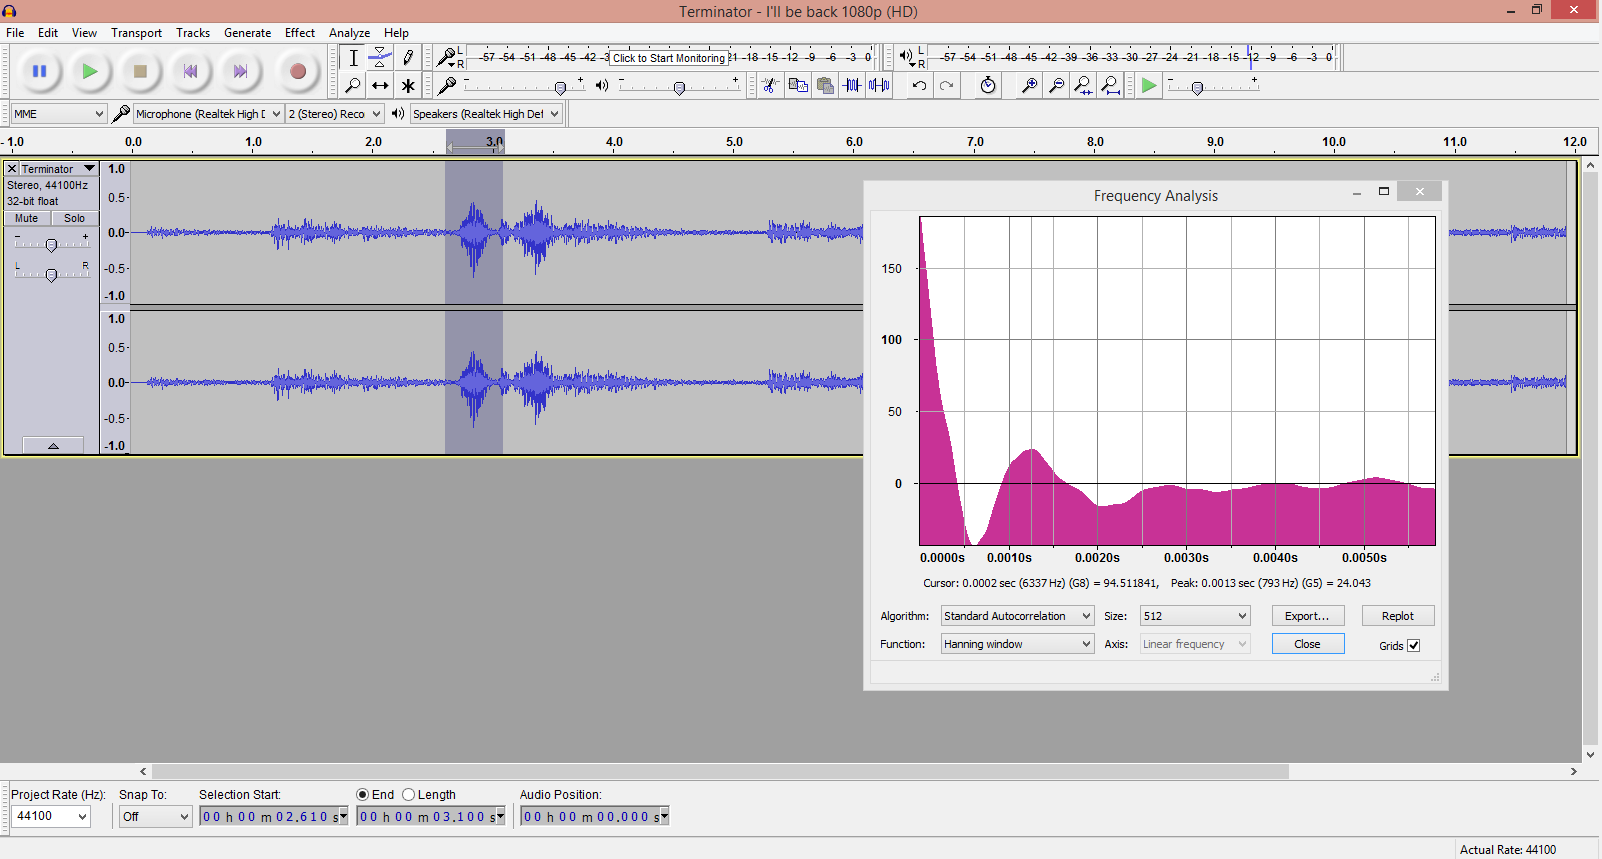
\includegraphics[width=1.0\textwidth]{autocorrelation2}
\caption{Vocal autocorrelation}
\end{figure}

Notice that the non-vocal graph tails out over the 5 millisecond window, whereas the vocal graph drops below zero and comes back up again within 1.5 ms, presumably because the human voice is more textured and contains more repeating patterns at shorter intervals than most other sounds, e.g. music.

\begin{todo}
Figure out how autocorrelation works.
\end{todo}

\begin{question}
Might we also be able to identify different voices?
\end{question}

It also looks like the same speaker has roughly the same graph, at least while speaking a single phrase, and different speakers have distinct graphs.

\end{document}
